\chapter{Mehrere Prädiktoren in einem Modell}\label{ch:multimod}
Wie wir es bereits in den letzten zwei Kapiteln
gesehen haben, kann das allgemeine lineare Modell
gut mit mehreren Prädiktoren umgehen. Von der
Berechnung her ändert sich hierbei eigentlich nichts.
Zu entscheiden, wann genau man mehrere Prädiktoren
in ein Modell aufnehmen sollte, ist aber nicht ganz ohne.
Weiter kann es oft schwierig sein, die geschätzten
Parameter richtig zu interpretieren.
Mit `interpretieren' sind hier keine fachlichen Interpretationen gemeint,
sondern rein statistische: Worauf beziehen sich die Zahlen
überhaupt?
In diesem Kapitel werden wir anhand von Simulationen
versuchen herauszufinden, wann es sinnvoll ist, mehrere
Prädiktoren in ein Modell aufzunehmen, wann dies mehr Nachteile
als Vorteile hat und was die geschätzten Parameter
überhaupt bedeuten.

\medskip

\begin{framed}
\textbf{Kausale Zusammenhänge.}
Die Parameterschätzungen, die das allgemeine lineare Modell liefert,
dienen in erster Linie der Beschreibung von Zusammenhängen in den Daten.
Öfters möchte man ihnen aber auch eine kausale Interpretation verleihen.
Zum Beispiel will man sich nicht damit begnügen, herauszufinden,
ob die Versuchspersonen in der Experimentalgruppe im Schnitt besser
abschneiden als jene in der Kontrollgruppe---man möchte wissen,
ob erstere im Schnitt besser abschneiden als letztere, eben \emph{weil}
sie zur Experimentalgruppe gehören.

{\bf Mit statistischen Techniken kann man Kausalität nicht nachweisen.}
Man kann aber Annahmen über die kausalen Zusammenhänge zwischen
den Variablen in einem Datensatz machen und sich dann überlegen,
wie man diese angenommenen Zusammenhänge am besten statistisch 
modelliert. Ob diese Annahmen berechtigt sind, ist dann 
eine Frage des Sachwissens und des Designs der Studie.
\end{framed}

\medskip

Ein nützliches Hilfsmittel beim Diskutieren angenommener
kausaler Zusammenhänge sind 
\textbf{\textit{directed acyclic graphs}},
kurz DAGs genannt. Diese werden in Lecture 1 im Skript
\href{https://janhove.github.io/teaching/2020/12/16/quant-meth}{\textit{Quantitative methodology: An introduction}} vorgestellt. Die grundsätzlich gleichen Infos 
finden sich bei \citet{Rohrer2018} und \citet{McElreath2020}. 
Es empfiehlt sich,
sich zur Vorbereitung dieses Kapitels eine dieser
Einführungen zur Brust zu nehmen.
Im Folgenden werden wir nämlich DAGs verwenden, um 
kausale Zusammenhänge zwischen ein paar Variablen
($x, y, z, \dots$) darzustellen. Von Interesse ist 
jeweils der kausale
Einfluss, den $x$ auf $y$ ausübt, zu schätzen. Die entscheidende
Fragen sind dann jeweils, ob dies überhaupt möglich ist und, wenn ja, ob
man hierzu noch Variablen ausser $x$ und $y$ ins Modell
aufnehmen sollte. 

\section{Störfaktoren berücksichtigen}\label{sec:störfaktoren}
Zunächst schauen wir uns das in Abbildung \ref{fig:dag1} dargestellte Szenario an.
Wir interessieren uns für den kausalen Einfluss von $x$ auf $y$,
aber die Möglichkeit besteht, dass eine weitere Variable $z$ sowohl $x$ als auch
$y$ beeinflusst. Wem dies lieber ist, der ersetze diese abstrakten Variablennamen
durch Bezeichnungen wie
\textit{Teilnahme an einem Kurs `Heimatsprache und -kultur'} (für $x$),
\textit{Ergebnis bei einem französischen Lesetest} (für $y$)
und \textit{sozioökonomischer Status des Elternpaars} (für $z$).
Aber meines Erachtens ist es unter dem Strich sinnvoller, sich mit der
Abstraktion anzufreunden, denn die Lektionen, die man aus diesen abstrakten
Szenarien ziehen kann, sind allgemeingültig.

\begin{knitrout}
\definecolor{shadecolor}{rgb}{0.969, 0.969, 0.969}\color{fgcolor}\begin{figure}
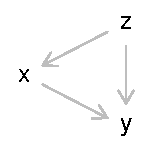
\includegraphics[width=.2\textwidth]{figure/unnamed-chunk-1-1} \caption{In diesem Szenario beeinflusst $z$ sowohl $x$ als auch $y$. Daher agiert $z$ als Störfaktor, wenn wir uns für den kausalen Zusammenhang zwischen $x$ und $y$ interessieren.\label{fig:dag1}}\label{fig:unnamed-chunk-1}
\end{figure}

\end{knitrout}

Wir machen nun dieses Szenario trotzdem etwas konkreter,
indem wir die Zusammenhänge zwischen den drei Variablen
in ein paar Gleichungen giessen.
Zunächst gehen wir der Einfachkeit halber davon aus,
dass die $z$-Variable aus einer Normalverteilung mit Mittel
0 und Standardabweichung 1 (also Varianz $1^2$) stammt.
Aber das ist eigentlich nicht so wichtig:
\begin{align}
z_i &\sim \textrm{Normal}(0, 1^2). \nonumber
\end{align}

Dann nehmen wir an, dass eine Zunahme von einer Einheit in der $z$-Variablen
eine Zunahme von 1.2 Einheiten in der $x$-Variablen bewirkt.
Es gibt aber noch Streuung in der $x$-Variablen, die nicht $z$ zugeschrieben
werden kann; diese Streuung erfassen wir durch einen Fehlerterm $\tau$
aus einer Normalverteilung mit Mittel 0 und Standardabweichung 1:
\begin{align}
x_i &= 0 + 1.2\cdot z_i + \tau_i, \label{eq:dag1_x} \\
\tau_i &\sim \textrm{Normal}(0, 1^2). \nonumber
\end{align}
Die Zahlen 1.2 in der ersten Zeile und 1 in der zweiten Zeile
wurden arbiträr gewählt. Die 0 in der ersten Zeile heisst lediglich,
dass das Mittel der $x$-Variablen 0 beträgt.

Weiter gehen wir in diesem Szenario davon aus,
dass die $y$-Variable durch die unten stehende Gleichung beschrieben wird.
Der kausale Einfluss von $x$ auf $y$ ist derart,
dass eine Zunahme von einer Einheit in $x$ eine Zunahme von 0.6 Einheiten
in $y$ bewirkt. Die Variable $z$ hat dahingegen eine negative Wirkung
auf $z$, aber für diese interessieren wir uns ja eigentlich nicht.
Die Zahlen $5.2$, $0.6$ und $-1.3$ sind wiederum arbiträr; Sie können hier auch
andere Zahlen verwenden.
\begin{align}
y_i &= 5.2 + 0.6\cdot x_i - 1.3 \cdot z_i + \varepsilon_i, \label{eq:dag1} \\
\varepsilon_i &\sim \textrm{Normal}(0, 1^2). \nonumber
\end{align}

Wir simulieren nun einen Datensatz mit 100 Beobachtungen dieser
drei Variablen. Wenn keine weiteren Parameter eingestellt werden,
generiert die Funktion \texttt{rnorm(n)} $n$ Beobachtungen aus einer
Normalverteilung mit Mittel 0 und Standardabweichung 1:
\begin{knitrout}
\definecolor{shadecolor}{rgb}{0.969, 0.969, 0.969}\color{fgcolor}\begin{kframe}
\begin{alltt}
\hlstd{n} \hlkwb{<-} \hlnum{100}
\hlstd{z} \hlkwb{<-} \hlkwd{rnorm}\hlstd{(n)}
\hlstd{x} \hlkwb{<-} \hlnum{0} \hlopt{+} \hlnum{1.2}\hlopt{*}\hlstd{z} \hlopt{+} \hlkwd{rnorm}\hlstd{(n)}
\hlstd{y} \hlkwb{<-} \hlnum{5.2} \hlopt{+} \hlnum{0.6}\hlopt{*}\hlstd{x} \hlopt{-} \hlnum{1.3}\hlopt{*}\hlstd{z} \hlopt{+} \hlkwd{rnorm}\hlstd{(n)}
\hlstd{d} \hlkwb{<-} \hlkwd{tibble}\hlstd{(y, x, z)}
\end{alltt}


{\ttfamily\noindent\bfseries\color{errorcolor}{\#\# Error in tibble(y, x, z): could not find function "{}tibble"{}}}\end{kframe}
\end{knitrout}

Um den Zusammenhang zwischen mehreren kontinuierlichen Variablen
aufs Mal grafisch darzustellen, bietet sich eine Streudiagrammmatrix
an. Unter
\url{https://janhove.github.io/RCode/scatterplot_matrix.R}
können Sie eine Funktion herunterladen, mit der ich selber Streu\-diagramm\-matrizen
zeichne. Sie basiert auf der \texttt{pairs()}-Funktion, die bereits in R
vorhanden ist.
Speichern Sie die Datei \texttt{scatterplot\_matrix.R} in einem neuen Subordner \texttt{functions}
in Ihrem R-Projekt. Sie können die Funktion dann wie folgt laden
und verwenden. Das Resultat und eine Erklärung über die Infos,
die dieser Streudiagrammmatrix zu entnehmen sind, finden Sie
in Abbildung \ref{fig:streudiagramm}. Weitere Infos im Blogeintrag
\href{https://janhove.github.io/reporting/2019/11/28/scatterplot-matrix}{\textit{Drawing scatterplot matrices
}} (28.11.2019).
\begin{knitrout}
\definecolor{shadecolor}{rgb}{0.969, 0.969, 0.969}\color{fgcolor}\begin{kframe}
\begin{alltt}
\hlkwd{source}\hlstd{(}\hlkwd{here}\hlstd{(}\hlstr{"functions"}\hlstd{,} \hlstr{"scatterplot_matrix.R"}\hlstd{))}
\end{alltt}


{\ttfamily\noindent\bfseries\color{errorcolor}{\#\# Error in here("{}functions"{}, "{}scatterplot\_matrix.R"{}): could not find function "{}here"{}}}\begin{alltt}
\hlkwd{scatterplot_matrix}\hlstd{(d)}
\end{alltt}


{\ttfamily\noindent\bfseries\color{errorcolor}{\#\# Error in scatterplot\_matrix(d): could not find function "{}scatterplot\_matrix"{}}}\end{kframe}
\end{knitrout}

Wir werden nun zwei Analysen miteinander vergleichen. Wenn wir
echte Daten analysieren würden, würden wir dies übrigens nicht tun: Wir
würden nur die sinnvollste Analyse ausführen. Aber das Ziel dieses
Kapitels ist es, herauszufinden, welche Analyse in Szenarien
wie diesem überhaupt die sinnvollste ist. Im ersten Modell
wird der Störfaktor ignoriert:
\begin{knitrout}
\definecolor{shadecolor}{rgb}{0.969, 0.969, 0.969}\color{fgcolor}\begin{kframe}
\begin{alltt}
\hlstd{dag1.lm1} \hlkwb{<-} \hlkwd{lm}\hlstd{(y} \hlopt{~} \hlstd{x,} \hlkwc{data} \hlstd{= d)}
\end{alltt}


{\ttfamily\noindent\bfseries\color{errorcolor}{\#\# Error in is.data.frame(data): object 'd' not found}}\begin{alltt}
\hlkwd{summary}\hlstd{(dag1.lm1)}\hlopt{$}\hlstd{coefficients}
\end{alltt}


{\ttfamily\noindent\bfseries\color{errorcolor}{\#\# Error in summary(dag1.lm1): object 'dag1.lm1' not found}}\end{kframe}
\end{knitrout}
% Die Parameterschätzungen dieses Modells sind zu interpretieren wie
% es in Abschnitt \vref{sec:regressioninterpretieren} erklärt wurde:
% \begin{itemize}
%  \item Nimmt man eine grosse Anzahl Beobachtungen, 
%  für die die $x$-Werte 0 sind, dann 
%  würde man laut diesem Modell erwarten, dass ihr $y$-Mittel $5.4 \pm 0.1$
%  beträgt.
%  \item Wenn man eine grosse Anzahl Beobachtungen,
%  für die die $x$-Werte 1 sind, mit einer grossen Anzahl
%  Beobachtungen, für die die $x$-Werte 0 sind, vergleicht,
%  dann würde man laut diesem Modell erwarten, dass das $y$-Mittel der ersten
%  Gruppe $0.11 \pm 0.07$ niedriger ist als das Mittel der zweiten Gruppe.
% \end{itemize}
% \emph{Mit dieser Interpretation gibt es kein Problem!}
% Man bemerke aber, dass wir in dieser Interpretation keine Kausalität implizieren.
% 
% Im zweiten Modell wird der Störfaktor berücksichtigt:
% <<>>=
% dag1.lm2 <- lm(y ~ x + z, data = d)
% summary(dag1.lm2)$coefficients
% @
% Auch die Parameterschätzung dieses Modells können wir interpretieren
% wie es in Abschnitt Abschnitt \ref{sec:regressioninterpretieren} erklärt wurde:
% \begin{itemize}
%  \item Nimmt man eine grosse Anzahl Beobachtungen, 
%  für die die $x$- und $z$-Werte beide 0 sind, dann 
%  würde man laut diesem Modell erwarten, dass ihr $y$-Mittel $5.4 \pm 0.1$
%  beträgt.
%  
%  \item Wenn man eine grosse Anzahl Beobachtungen,
%  für die die $x$-Werte 1 und die $z$-Werte 0 sind, mit einer grossen Anzahl
%  Beobachtungen, für die die $x$- und $z$-Werte beide 0 sind, vergleicht,
%  dann würde man laut diesem Modell erwarten, dass das $y$-Mittel der ersten
%  Gruppe $0.54 \pm 0.11$ höher ist als das Mittel der zweiten Gruppe.
%  
%  \item Wenn man eine grosse Anzahl Beobachtungen,
%  für die die $z$-Werte 1 und die $x$-Werte 0 sind, mit einer grossen Anzahl
%  Beobachtungen, für die die $x$- und $z$-Werte beide 0 sind, vergleicht,
%  dann würde man laut diesem Modell erwarten, dass das $y$-Mittel der ersten
%  Gruppe $1.2 \pm 0.2$ niedriger ist als das Mittel der zweiten Gruppe.
% \end{itemize}
% Der zweite Punkt widerspricht der Interpretation des ersten Modells \emph{nicht}:
% Nur weil die Parameter in den Modellen zum Teil gleich heissen (\texttt{(Intercept)},
% \texttt{x}), bedeutet das noch nicht, dass sie gleich zu interpretieren sind.
% Im zweiten Modell kann man den geschätzten \texttt{x}-Parameter nicht interpretieren,
% ohne die ins Modell aufgenommene $z$-Variable zu berücksichtigen;
% im ersten Modell muss man den geschätzten \texttt{x}-Parameter interpretieren,
% ohne die nicht im Modell vorhandene $z$-Variable zu berücksichtigen!
% 
% Wenn man die geschätzten Parameter des zweiten Modells mit Gleichung \vref{eq:dag1}
% vergleicht, sieht man, dass das zweite Modell die Parameter aus dieser
% Gleichung in etwa richtig schätzt. Tatsächlich sind die Unterschiede zwischen
% den Parameterschätzungen des Modells und den Parameter aus der Gleichung
% rein zufallsbedingt und ausserdem schätzt das Modell diese Parameter im Schnitt
% ohne Verzerrung. Wenn man dies genauer überprüfen möchte, kann man eine Simulation
% programmieren, in der man anhand von Gleichungen \ref{eq:dag1_x} und \ref{eq:dag1}
% ein paar tausend Datensätze generiert und diese analysiert.
% Die Funktion \texttt{generate\_dag1()} generiert defaultmässig
% 10'000 solche Datensätze mit je 100 Beobachtungen
% und analysiert diese mal wie im ersten Modell (ohne $z$)
% und mal wie im zweiten Modell (mit $z$). Für jede Stichprobe und jedes Modell
% wird die Schätzung des \texttt{x}-Parameters gespeichert und ausgegeben.
% 
% <<>>=
% generate_dag1 <- function(
%   n = 100,      # Anzahl Datenpunkte
%   sims = 10000, # Anzahl Simulationen
%   z_x = 1.2,    # Effekt z -> x
%   x_y = 0.6,    # Effekt x -> y
%   z_y = -1.3    # Effekt z -> y
% ) {
%   est_lm1 <- vector(length = sims)
%   est_lm2 <- vector(length = sims)
%   
%   for (i in 1:sims) {
%     z <- rnorm(n)
%     x <- 0 + z_x*z + rnorm(n)
%     y <- 5.2 + x_y*x + z_y*z + rnorm(n)
%     mod.lm1 <- lm(y ~ x)
%     mod.lm2 <- lm(y ~ x + z)
%     est_lm1[[i]] <- coef(mod.lm1)[[2]]
%     est_lm2[[i]] <- coef(mod.lm2)[[2]]
%   }
%   
%   return(tibble(`Modell 1` = est_lm1, 
%                 `Modell 2` = est_lm2))
% }
% @
% 
% Wir lassen die Funktion mit den Defaulteinstellungen laufen
% und stellen die Schätzung des \texttt{x}-Parameters in beiden
% Modellen dar (Abbildung \ref{fig:schätzung_dag1}).
% <<cache = TRUE, fig.cap="Modell 2, das den Störfaktor $z$ berücksichtigt, liefert eine unverzerrte Schätzung des Parameters, der den Einfluss von $x$ auf $y$ in Gleichung \\ref{fig:dag1} ausdrückt (0.6). Modell 1 liefert aber eine verzerrte Schätzung dieses Parameters. Je nach den in Gleichungen \\ref{eq:dag1_x} und \\ref{eq:dag1} gewählten Parameterwerten wird diese Verzerrung eine Über- oder Unterschätzung sein; hier handelt es sich um eine Unterschätzung.\\label{fig:schätzung_dag1}">>=
% est_dag1 <- generate_dag1()
% 
% est_dag1 %>% 
%   pivot_longer(cols = everything(),
%                names_to = "Modell",
%                values_to = "Schätzung") %>% 
%   ggplot(aes(x = Schätzung)) +
%   geom_histogram(bins = 50,
%                  fill = "grey", colour = "black") +
%   facet_grid(. ~ Modell) +
%   xlab("Schätzung x -> y") +
%   ylab("Anzahl")
% @
% 
% Die Simulation bestätigt, dass Modell 2, aber nicht Modell 1, 
% eine unverzerrte Schätzung
% des kausalen Einflusses von $x$ auf $y$ liefert (0.6):
% <<>>=
% apply(est_dag1, 2, mean)
% @
% 
% \medskip
% 
% \begin{framed}
% Das Modell ohne den Störfaktor ist nicht falsch.
% Wenn man sich für die Frage interessiert, wie gross
% der durchschnittliche Unterschied in der $y$-Variablen
% ist, wenn Beobachtungen vergleicht, die sich um eine
% Einheit in der $x$-Variablen unterscheiden, ist dieses
% Modell genau, was man braucht.
% Aber die Schätzungen dieses Modells kann man nicht
% kausal interpretieren, wenn man von den kausalen
% Zusammenhängen in Abbildung \ref{fig:dag1} ausgeht.
% \end{framed}
% 
% \medskip
% 
% Das Fazit der obigen Betrachtungen scheint klar:
% Wenn man vermutet, dass Störfaktoren im Spiel sind,
% sollte man diese in der Analyse berücksichtigen,
% wenn man kausale Einflüsse schätzen will.
% In der Praxis ist dies aber nicht so einfach.
% Erstens setzt dieser Ansatz voraus, dass wir
% alle Störfaktoren kennen und überhaupt berücksichtigen
% können. Zweitens sind unsere Messungen nicht perfekt.
% Und drittens ist es möglich, dass die Störfaktoren
% einen nichtlinearen Effekt ausüben, während wir 
% oben nur lineare Effekte berücksichtigt haben.
% Die Konsequenzen der ersten beiden Umstände können Sie
% in den folgenden fakultativen Aufgaben genauer unter
% die Lupe nehmen. Das Fazit verrate ich Ihnen schon:
% 
% \medskip
% 
% \begin{framed}
% \textbf{Machen Sie sich keine Hoffnung, dass Sie mit statistischen
% Mitteln den Einfluss von Störfaktoren angemessen berücksichtigen können.}
% Dazu müssten Sie nämlich alle Störfaktoren kennen, diese perfekt
% gemessen haben und die funktionale Form ihrer kausalen Einfluss richtig
% spezifizieren.
% \textbf{Statistische Mittel sind kein Ersatz für ein solides Forschungsdesign, 
% das Störfaktoren neutralisiert.}
% \end{framed}
% 
% \paragraph{Aufgabe 1: Unbekannte Störfaktoren}
% In Abbildung \ref{fig:dag1_aufgabe1} wurde unser DAG 
% um einen Störfaktor $u$ erweitert. Dieser Störfaktor 
% ist aber unbekannt oder kann aus irgendwelchen Gründen
% nicht erhoben werden. Wir gehen von den folgenden kausalen
% Gleichungen aus:
% \begin{align*}
% z_i &\sim \textrm{Normal}(0, 1^2),  \\
% u_i &\sim \textrm{Normal}(0, 1^2), \\
% x_i &= 0 + 1.2\cdot z_i + 0.9\cdot u_i + \tau_i, \\
% y_i &= 5.2 + 0.6\cdot x_i - 1.3 \cdot z_i + 2.5\cdot u_i + \varepsilon_i,\\
% \tau_i &\sim \textrm{Normal}(0, 1^2),  \\
% \varepsilon_i &\sim \textrm{Normal}(0, 1^2). 
% \end{align*}
% Einen Datensatz mit 50 Beobachtungen können wir wie folgt generieren.
% Bemerken Sie, dass die Variable $u$ zwar kreiert wird, aber nicht dem Datensatz hinzugefügt wird:
% Sie beeinflusst die $x$- und $y$-Variablen, aber wurde in der simulierten Studie ja nicht erhoben.
% <<>>=
% n <- 50
% z <- rnorm(n)
% u <- rnorm(n)
% x <- 0 + 1.2*z + 0.9*u + rnorm(n)
% y <- 5.2 + 0.6*x - 1.3*z + 2.5*u + rnorm(n)
% d <- tibble(y, x, z)
% @
% 
% <<message = FALSE, fig.width=1, fig.height=1, out.width=".2\\textwidth", echo = FALSE, fig.cap="Der Störfaktor $z$ ist im Datensatz vorhanden, aber der Störfaktor $u$ wurde nicht erhoben.\\label{fig:dag1_aufgabe1}">>=
% dag1 <- dagitty("dag {
%    z -> x
%    z -> y
%    x -> y
%    u -> x
%    u -> y
%    u[unobserved]
% }")
% coordinates(dag1) <- list(
%   y = c(x = 2, y = 2, z = 0, u = 0),
%   x = c(x = 0, y = 1, z = 1, u = 0)
% )
% drawdag(dag1)
% @
% 
% Wir könnten nun ein Modell rechnen, 
% in dem immerhin der Störfaktor $z$ aufgenommen wurde:
% <<>>=
% aufgabe1.lm <- lm(y ~ x + z, data = d)
% summary(aufgabe1.lm)$coefficients
% @
% \begin{enumerate}
%   \item Erklären Sie haargenau, was die Parameterschätzung für \texttt{x} bedeutet.
%   \item Zeigen Sie anhand einer Simulation, dass das Modell \texttt{aufgabe1.lm} keine
%   unverzerrte Schätzung des kausalen Einflusses von $x$ auf $y$ liefert, obwohl der Störfaktor $z$
%   berücksichtigt wurde.
%   \item Würde sich die Situation verbessern, wenn wir mit Datensätzen von 200 statt von 50 Beobachtungen
%   arbeiten würden?
% \end{enumerate}
% 
% \paragraph{Aufgabe 2: Messfehler im Störfaktor}
% Abbildung \ref{fig:dag1_aufgabe2} zeigt ein Szenario,
% wo $z$ ein Störfaktor im Zusammenhang von $x$ und $y$ ist,
% aber wo wir $z$ selber nicht gemessen haben.
% Stattdessen haben wir einen \textbf{Indikator} von $z$ gemessen.
% Dieser widerspiegelt das \textbf{Konstrukt} ($z$) imperfekt.
% Dass man Konstrukte (z.B.\ Arbeitsgedächtnis, L2-Schreibfähigkeit, L1-Vokabelwissen, Intelligenz, sozioökonomischer Status usw.)
% nur imperfekt misst, ist eher die Regel als die Ausnahme.
% Es ist aber wichtig, zu verstehen, wie sich diesen Messfehler
% auf die statistische Kontrolle auswirkt; siehe dazu auch Lecture 9 im Skript \href{https://janhove.github.io/teaching/2020/12/16/quant-meth}{\textit{Quantitative methodology: An introduction}}.
% 
% Wir übernehmen die kausalen Gleichungen aus dem Anfang dieses
% Abschnitts: $x$ beeinflusst $y$ und $z$ beeinflusst sowohl
% $x$ als auch $y$. Der Unterschied besteht darin, dass wir 
% statt $z$ nun $z_m$ beobachten. Die gemessene Variable
% $z_m$ setzt sich zusammen aus dem Konstrukt $z$
% und einem Messfehler $\psi$, der aus einer Normalverteilung
% mit Mittel 0 und Standardabweichung 0.3 (also Varianz $0.3^2$) 
% stammt.
% \begin{align}
% z_i &\sim \textrm{Normal}(0, 1^2), \nonumber \\
% z_{m,i} &= z_i + \psi_i, \nonumber \\
% x_i &= 0 + 1.2\cdot z_i + \tau_i, \nonumber \\
% y_i &= 5.2 + 0.6\cdot x_i - 1.3 \cdot z_i + \varepsilon_i, \nonumber \\
% \psi_i &\sim \textrm{Normal}(0, 0.3^2), \label{eq:dag1_aufgabe2}\\
% \tau_i &\sim \textrm{Normal}(0, 1^2),  \nonumber \\
% \varepsilon_i &\sim \textrm{Normal}(0, 1^2). \nonumber
% \end{align}
% 
% <<message = FALSE, fig.width=1, fig.height=1, out.width=".2\\textwidth", echo = FALSE, fig.cap="Es gibt im kausalen Zusammenhang zwischen $x$ und $y$ einen Störfaktor $z$, aber dieser wurde nicht direkt erhoben. Stattdessen müssen wir uns mit einem Indikator $z_m$ begnügen.\\label{fig:dag1_aufgabe2}">>=
% dag1 <- dagitty("dag {
%    z -> x
%    z -> y
%    x -> y
%    z[unobserved]
%    z -> z_m
% }")
% coordinates(dag1) <- list(
%   y = c(x = 2, y = 2, z = 0, z_m = 0),
%   x = c(x = 0, y = 1, z = 0, z_m = 1)
% )
% drawdag(dag1)
% @
% 
% In R können wir 50 Beobachtungen dieser Variablen wie folgt
% simulieren. Beachten Sie, dass $z$ dem Datensatz nicht hinzugefügt
% wird, da wir statt $z$ $z_m$ gemessen haben.
% <<>>=
% n <- 50
% z <- rnorm(n)
% z_m <- z + rnorm(n, sd = 0.3)
% x <- 0 + 1.2*z + rnorm(n)
% y <- 5.2 + 0.6*x - 1.3*z + rnorm(n)
% d <- tibble(y, x, z_m)
% @
% 
% Statt $z$ können wir nur $z_m$ in der Analyse berücksichtigen:
% <<>>=
% aufgabe2.lm <- lm(y ~ x + z_m, data = d)
% summary(aufgabe2.lm)$coefficients
% @
% 
% \begin{enumerate}
%   \item Erklären Sie haargenau, was die Parameterschätzung für \texttt{x} bedeutet.
%   \item Zeigen Sie anhand einer Simulation, dass das Modell \texttt{aufgabe2.lm} keine
%   unverzerrte Schätzung des kausalen Einflusses von $x$ auf $y$ liefert, obwohl der Störfaktor $z$
%   mit einem Indikator $z_m$ berücksichtigt wurde.
%   \item Würde sich die Situation verbessern, wenn wir mit Datensätzen von 200 statt von 50 Beobachtungen
%   arbeiten würden?
%   \item Wäre es besser, den Störfaktor $z$ in keinerlei Weise
%   zu berücksichtigen?
%   \item Würde sich die Situation verbessern, wenn wir über einen 
%   genaueren Indikator von $z$ verfügten? Wiederholen Sie
%   zur Beantwortung dieser Frage die Simulation, aber
%   verwenden Sie für $\psi$ in Gleichung \ref{eq:dag1_aufgabe2}
%   eine Standardabweichung von 0.1 statt 0.3.
% \end{enumerate}
% % 
% % \paragraph{Aufgabe 3: Nichtlinearer Effekt des Störfaktors}
% % 
% % <<>>=
% % n <- 100
% % z <- rnorm(n)
% % x <- 0 + 1.2*z + rnorm(n)
% % y <- 5.2 + 0.6*x - 1.3*I(z^2) + rnorm(n)
% % d <- tibble(y, x, z)
% % @
% % 
% % \medskip
% % 
% % \begin{framed}
% % \textbf{Fazit Störfaktoren.}
% % 
% % \end{framed}
% 
% \section{Kontrollvariablen bei kontrollierten Experimenten}\label{sec:kontrollvariablen}
% In Abschnitt \ref{sec:störfaktoren} haben wir das Szenario behandelt, in dem
% die Drittvariable $z$ sowohl $x$ als auch $y$ beeinflusst. Dieses Szenario ist
% typisch für sog.\ observationelle (oder korrelationelle) Studien und Quasi-Experimente.
% In diesem Abschnitt behandeln wir dahingegen kontrollierte Experimente, in denen
% die Werte von $x$ nach dem Zufallsprinzip von den Forschenden manipuliert wurden.
% In Abbildung \ref{fig:dag2} wird das $x$ daher als $x_r$ dargestellt ($r$ für \textit{randomised}).
% Ein typisches Beispiel für das hier betrachtete abstrakte Szenario ist die zufällige Zuordnung von Versuchspersonen
% zu den Konditionen eines Experiments. 
% In diesem Fall wäre $x$ eine kategorielle
% Variable, aber ohne Beschränkung der Allgemeinheit werden wir uns hier für kontinuierliche
% $x$-Variablen interessieren. Das vereinfacht nur die Simulationen; an den Schlussfolgerungen
% ändert dies nichts.
% Die Variable $z$ wäre dann eine Variable, für die man sich zwar in erster Linie nicht interessiert,
% aber von der man vermutet, dass sie mit der abhängigen Variablen ($y$) korreliert ist.
% Das Paradebeispiel hierfür ist ein Prätest/Posttest-Experiment, wo $x$ die Rolle der Kondition übernimmt,
% $y$ die Posttestergebnisse darstellt und $z$ die Prätestergebnisse.
% 
% <<message = FALSE, fig.width=1, fig.height=1, out.width=".2\\textwidth", echo = FALSE, fig.cap="In diesem Szenario wurden die $x$-Werte zufällig und unabhängig von $z$ zugewiesen. Dies wäre typisch für kontrollierte Experimente, in denen die unabhängige Variable $x$ von den Forschenden nach dem Zufallsprinzip manipuliert wird.\\label{fig:dag2}">>=
% dag2 <- dagitty("dag {
%    z -> y
%    x_r -> y
% }")
% coordinates(dag2) <- list(
%   y = c(x_r = 1, y = 2, z = 0),
%   x = c(x_r = 0, y = 1, z = 1)
% )
% drawdag(dag2)
% @
% 
% Für die Simulationen gehen wir von dem von den folgenden Gleichungen
% beschriebenen Mechanismus aus:
% \begin{align}
% x_i &\sim \textrm{Normal}(0, 1^2), \nonumber \\
% z_i &\sim \textrm{Normal}(0, 1^2), \nonumber \\
% y_i &= 5.2 + 0.3\cdot x_i + 0.9 \cdot z_i + \varepsilon_i, \label{eq:dag2} \\
% \varepsilon_i &\sim \textrm{Normal}(0, 1^2). \nonumber
% \end{align}
% 
% In R können wir einen Datensatz mit 100 Beobachtungen, die diesen Gleichungen entsprechen,
% wie folgt kreieren:
% <<>>=
% n <- 100
% x <- rnorm(n)
% z <- rnorm(n)
% y <- 5.2 + 0.3*x + 0.9*z + rnorm(n)
% d <- tibble(y, x, z)
% @
% 
% <<eval = FALSE>>=
% # Streudiagrammmatrix nicht im Skript
% scatterplot_matrix(d)
% @
% 
% Wiederum rechnen wir ein Modell ohne und eins mit der $z$-Variablen.
% Man bemerke, dass zumindest für diese simulierten Daten beide Modell recht ähnliche 
% Schätzungen für den \texttt{x}-Parameter liefern: $0.36 \pm 0.15$ und $0.36 \pm 0.11$.
% <<>>=
% dag2.lm1 <- lm(y ~ x, data = d)
% summary(dag2.lm1)$coefficients
% 
% dag2.lm2 <- lm(y ~ x + z, data = d)
% summary(dag2.lm2)$coefficients
% @
% 
% Tatsächlich liefern \emph{beide} Modelle eine unverzerrte Schätzung des kausalen Einflusses
% von $x$ auf $y$. Keines der Modelle ist also schlecht. Trotzdem ist das zweite Modell,
% in dem die $z$-Variable mitberücksichtigt wird, das Modell, das man rechnen sollte,
% wenn man überhaupt über die $z$-Variable verfügt. Der Grund dafür wird klarer, wenn
% wir wieder ein paar tausend Datensätze generieren.
% Dafür könnten 
% wir zwar eine neue Funktion \texttt{generate\_dag2()}
% schreiben. Aber wenn wir der Funktion \texttt{generate\_dag1()}
% den Parameterwert 0 für \texttt{z\_x}
% übergeben, erhalten wir auch die gewünschten Datensätze:
% <<cache = TRUE>>=
% est_dag2 <- generate_dag1(x_y = 0.3, z_y = 0.9, z_x = 0)
% @
% 
% Wie Abbildung \ref{fig:schätzung_dag2} zeigt, liefern beide Modelle unverzerrte
% Schätzungen des kausalen Einflusses von $x$ auf $y$ aus Gleichung \ref{eq:dag2}.
% Die Schätzungen von Modell 2 variieren aber weniger von Datensatz zu Datensatz,
% das heisst, sie liegen im Schnitt näher bei dem eigentlichen Wert.
% <<cache = TRUE, fig.cap="Beide Modelle liefern unverzerrte Schätzungen des Parameters, der den Einfluss von $x$ auf $y$ in Gleichung \\ref{eq:dag2} ausdrückt (0.3). Die Schätzungen von Modell 2 variieren aber weniger zwischen den simulierten Datensätzen, das heisst, sie sind im Schnitt genauer.\\label{fig:schätzung_dag2}">>=
% est_dag2 %>% 
%   pivot_longer(cols = everything(),
%                names_to = "Modell",
%                values_to = "Schätzung") %>% 
%   ggplot(aes(x = Schätzung)) +
%   geom_histogram(bins = 50,
%                  fill = "grey", colour = "black") +
%   facet_grid(. ~ Modell) +
%   xlab("Schätzung x -> y") +
%   ylab("Anzahl")
% @
% 
% Eine numerische Kontrolle bestätigt dies. Die Mittel der beiden
% Verteilungen sind nahezu gleich und nur wegen der beschränkten Anzahl
% Simulationen nicht genau 0.3. Verglichen zu den Schätzungen von Modell 1
% haben die Schätzungen von Modell 2 aber eine Standardabweichung, die etwa
% 25\% niedriger ist:
% <<>>=
% apply(est_dag2, 2, mean)
% apply(est_dag2, 2, sd)
% @
% 
% \paragraph{Fazit} 
% Die Genauigkeit, mit der ein Modellparameter geschätzt
% wird, hängt von der Datenmenge und der Fehlervarianz ab.
% Dies zeigte sich bereits in der Formel zur Berechnung
% des Standardfehlers eines Mittels
% ($\widehat{\textrm{SE}} = \frac{s}{\sqrt{n}}$).
% Die Genauigkeit kann man also erhöhen, indem man
% mehr Daten sammelt oder indem man die Fehlervarianz senkt.
% Letzteres kann man wiederum auf ein paar Arten und Weisen bewirken:
% 
% \begin{itemize}
%  \item indem man zuverlässigere Instrumente, die das Konstrukt, für das
%  man sich interessiert, genauer messen, verwendet;
%  
%  \item indem man den Einfluss von weiteren Variablen auf die outcome-Variable
%  im Design der Studie reduziert. Wenn Alter ein möglicher Faktor wäre, 
%  könnte man zum Beispiel nur Teilnehmende in einer bestimmten 
%  schmalen Altersspanne rekrutieren.
%  Hier muss man natürlich eine Abwägung zwischen der Genauigkeit der Ergebnisse
%  und ihrer Generalisierbarkeit machen.
%  
%  \item indem man den Einfluss solcher weiteren Variablen
%  statistisch berücksichtigt.
% \end{itemize}
% 
% In dem wir die Drittvariable $z$ ins Modell aufnehmen, obwohl sie
% keinen Störfaktor im Zusammenhang zwischen $x$ und $y$ darstellt,
% wird die Fehlervarianz kleiner und die Genauigkeit der Schätzungen
% grösser.
% Auch wenn Ihnen
% der Einfluss irgendeiner Variablen egal ist, kann es sich daher lohnen, diese Variable
% trotzdem mitzuerheben, wenn sie den Restfehler eingreifend reduzieren kann, insbesondere
% wenn die zusätzliche Variable leicht zu erheben ist.
% 
% \medskip
% 
% \begin{framed}
% \textbf{Auch in kontrollierten Experimenten lohnt es sich, wichtige Kontrollvariablen in der Analyse zu berücksichtigen.}
% Der Grund ist nicht, dass man eine verzerrte Schätzung vorbeugen will---auch ohne Kontrollvariablen 
% würde das Modell eine unverzerrte Schätzung liefern.
% Vielmehr ist der Grund, dass man die Genauigkeit der Schätzung dadurch erhöhen kann.
% Dieser Vorteil trifft übrigens auch dann zu, und sogar \emph{besonders} dann, wenn
% die Kontrollvariablen ($z$) nicht mit der unabhängigen Variablen ($x$) korreliert ist.
% 
% Übertreiben Sie aber nicht mit der Anzahl Kontrollvariablen. Eine oder zwei Kontrollvariablen,
% von denen man im Vorfeld weiss, dass sie stark mit dem outcome, aber kaum miteinander,
% korrelieren werden, und die man auch \emph{vor} der Intervention erheben kann, sind nützlicher als eine grosse
% Anzahl von Kontrollvariablen, die vielleicht je nach Wetterlage und Mondposition
% einen Einfluss haben könnten. Insbesondere Prätestergebnisse sind wertvolle Kontrollvariablen,
% da sie in der Regel stark mit den Posttestergebnissen kontrollieren und weder von der Intervention
% betroffen sind noch die Gruppenzugehörigkeit bei der Intervention kausal beeinflussen.
% \end{framed}
% 
% \paragraph{Beispiel Analyse Prätest/Posttestexperiment}
% Aus den Überlegungen in diesem Abschnitt folgt, dass
% die Standardanalyse eines Prätest/Posttestexperiments mit 
% kontinuierlichen Posttestergebnissen recht einfach ist:
% <<eval = FALSE>>=
% mod.lm <- lm(posttest ~ kondition + pretest, data = d)
% @
% Von Interesse wäre dann die Schätzung des \texttt{kondition}-Parameters.
% Diese Analyse wollen wir nun an einem Beispiel illustrieren.
% Die Daten, die wir analysieren werden, stammen
%   aus einer Studie von \citet{Mueller2020}, in der bei 260 Kindern
%   untersucht wurde, wie gut diese deutsch--englische Kognatwörter
%   lernen konnten. Es fanden drei Datenerhebungen statt: T1, T2 und T3.
%   Nach der ersten Datenerhebung wurde mit 120 Kindern eine Intervention
%   durchgeführt, die zum Ziel hatte, den Kindern ein grösseres Bewusstsein
%   für Kognatkorrespondenzen beizubringen. Die anderen 140 Kinder dienten
%   als Kontrollgruppe.
%   
%   Wir interessieren uns hier für die Frage, ob die Intervention dazu führte,
%   dass die Kinder besser deutsch--englische Kognatwörter lernen. 
%   Wir tun hier, als ob die Kinder zufällig und unabhängig voneinander
%   den Konditionen zugeordnet wurden. Das war zwar nicht der Fall \citep[][S.~27]{Mueller2020},
%   aber das Ziel hier ist es, zu zeigen, wie die Standardanalyse in 
%   diesem Ideallfall aussähe.
%   Wir interessieren uns für die Posttestergebnisse bei der dritten Erhebung (T3);
%   die Prätestergebnisse dienen uns als Kontrollvariable (T1);
%   die Messungen der zweiten Erhebung ignorieren wir.
%   
%   Lesen wir zunächst die Daten ein. Wir behalten der Übersichtlichkeit
%   halber nur die Spalten, die wir tatsächlich brauchen.
% <<message = FALSE, warning = FALSE>>=
% d <- read_csv(here("data", "mueller_datacorr.csv")) %>% 
%   select(ID, Class, Group, T1cog, T3cog)
% @
% Eine Möglichkeit, die Daten grafisch darzustellen, ist in einem
% Streudiagramm, in dem die Datenpunkte je nach Kondition eine
% andere Farbe haben. Mit \texttt{geom\_smooth()} können wir pro Kondition
% eine Trendlinie hinzufügen. Man bemerke, dass für beliebige Prätestwerte
% die Interventionsgruppe im Schnitt besser abzuscheiden scheint als
% die Kontrollgruppe (Abbildung \ref{fig:mueller1}).
% <<message = FALSE, fig.cap="Individuelle T3- vs. T1-Ergebnisse bei \\citet{Mueller2020}.\\label{fig:mueller1}">>=
% ggplot(d,
%        aes(x = T1cog, y = T3cog,
%            colour = Group)) +
%   geom_point(shape = 1) +
%   geom_smooth(method = "lm", se = FALSE) +
%   xlab("Prätestergebnisse") +
%   ylab("Posttestergebnisse")
% @
% Wir können, wie bereits erwähnt, ein recht einfaches Modell rechnen,
% um den Interventionseffekt zu schätzen:
% <<eval = TRUE>>=
% mueller.lm <- lm(T3cog ~ Group + T1cog, data = d)
% @
% Um das Intercept etwa informativer zu machen, können wir 
% \textit{sum-coding} auf \texttt{Group} anwenden (siehe Abschnitt \vref{sec:sumcoding})
% und die Kontrollvariable um ihr Mittel zentrieren. Das Intercept
% stellt dann das erwartete durchschnittliche Ergebnis zu T3
% bei Versuchspersonen mit einem durchschnittlichen T1-Ergebnis
% dar, über die beiden Konditionen des Experiments hinweg.
% Diese Schritte sind aber optional; nur die Interpretation des Intercepts
% ändert sich hierdurch.
% <<>>=
% d$n.Group <- ifelse(d$Group == "intervention", 0.5, -0.5)
% d$c.T1cog <- d$T1cog - mean(d$T1cog)
% mueller.lm <- lm(T3cog ~ n.Group + c.T1cog,
%                  data = d)
% summary(mueller.lm)$coefficients
% @
% Diese Analyse liefert eine Schätzung des Interventionseffekt
% von $2.2 \pm 0.5$ Punkten zugunsten der Interventionsgruppe.
% 
% Bemerken Sie, dass wir nirgends davon ausgegangen sind,
% dass die Prä- und Posttest identisch oder auch nur ähnlich waren.
% Tatsächlich hätte die Analyse gleich ausgesehen, auch wenn
% die Kontrollvariable kein Prätestergebnis, sondern etwa
% ein IQ-Score oder eine Selbstbeurteilung, die vor der Intervention
% erhoben wurde, gewesen wäre.
% 
% Bemerken Sie weiter, dass die Schätzung für \texttt{c.T1cog} 
% \emph{uns nicht interessiert}. Wir brauchen diesen Parameter,
% um die Genauigkeit der Parameterschätzung für \texttt{n.Group}
% zu erhöhen, aber dass die Posttestergebnisse positiv
% mit den Prätestergebnissen ist nicht relevant für 
% die Forschungsfrage.
% 
% Tatsächlich wurden die Kinder in der Studie von \citet{Mueller2020}
% aber nicht nach dem Zufallsprinzip und unabhängig voneinander
% den Konditionen zugeordnet. Stattdessen wurden sie per Schulklasse
% zugeordnet, und auch diese Zuordnung erfolgte nicht nach
% dem Zufallsprinzip:
% \begin{quote}
% ``Based on the number of lessons they were able to dedicate
% to the project, 10 classes were assigned to the [control group]
% and seven classes to the [intervention group].'' \citep[][S.~27]{Mueller2020}
% \end{quote}
% Entgegen den Tatsachen werden wir jetzt tun, als ob die Kinder zwar
% in ganzen Klassen, aber schon nach dem Zufallsprinzip den Konditionen
% zugeordnet wurden. Das heisst, wir tun jetzt, als ob die vorliegenden
% Daten aus einem \textit{cluster-randomised experiment} kommen.
% Das Ziel ist es, zu zeigen, wie man Daten aus solchen Experimenten
% auf eine recht einfache aber korrekte Art und Weise analysieren kann.
% Für weitere Details verweise ich auf \citet{Vanhove2015,Vanhove2020c}.
% 
% Dass die Kinder nicht unabhängig voneinander, sondern in ganzen Klassen
% den Konditionen zugeordnet wurden, müssen wir unbedingt in der Analyse
% berücksichtigen. Eine einfache Art und Weise, dies zu tun, besteht darin,
% pro Klasse den Durchschnitt des \textit{outcomes} und der Kontrollvariablen
% zu berechnen. Statt mit den individuellen Daten zu rechnen, rechnen wir
% mit diesen Klassendurchschnitten weiter. Abbildung \ref{fig:mueller2}
% zeigt das resultierende Streudiagramm.
% <<message = FALSE, fig.cap="Durchschnittliche T3- vs. T1-Ergebnisse pro Klasse bei \\citet{Mueller2020}.\\label{fig:mueller2}">>=
% d_per_class <- d %>% 
%   group_by(Class, Group) %>% 
%   summarise(
%     mean_T1 = mean(T1cog),
%     mean_T3 = mean(T3cog),
%     n = n(),
%     .groups = "drop"
%   )
% ggplot(d_per_class,
%        aes(x = mean_T1, y = mean_T3,
%            colour = Group)) +
%   geom_point(shape = 1) +
%   geom_smooth(method = "lm", se = TRUE) +
%   xlab("Klassendurchschnitt\nPrätest") +
%   ylab("Klassendurchschnitt\nPosttest")
% @
% Über die Tatsache, dass die 
% Trendlinien nicht schön parallel verlaufen wie in Abbildung \ref{fig:mueller1}
% würde ich mir keine grossen Sorgen machen. Dies könnte dennoch darauf hindeuten,
% dass die Intervention relativ stärker wirkt in Klassen, die im Schnitt
% beim Prätest schlechter abschnitten. Diese Möglichkeit untersuchen Sie
% genauer in den Aufgaben am Schluss dieses Kapitels.\label{page:mueller}
% <<>>=
% mueller_class.lm <- lm(mean_T3 ~ Group + mean_T1,
%                        data = d_per_class)
% summary(mueller_class.lm)$coefficients
% @
% Diese Analyse, in der von einer zufälligen Zuordnung auf Klassenebene
% ausgegangen wird, ergibt einen geschätzten Interventionseffekt von
% $2.2 \pm 0.7$ Punkten. Obwohl der Standardfehler um die Schätzung
% grösser ist als in der ersten Analyse, ist diese Analyse zu bevorzugen,
% da sie der Tatsache Rechnung trägt, dass die Versuchspersonen nicht
% unabhängig voneinander den Konditionen zugewiesen wurden.
% 
% \section{Vorsicht bei \textit{posttreatment}-Variablen}
% In Abschnitt \ref{sec:störfaktoren} beeinflusste die Drittvariable
% $z$ sowohl $x$ als auch $y$; in Abschnitt \ref{sec:kontrollvariablen}
% beeinflusste $z$ nur $y$ und wurde sie auch nicht von $x$ beeinflusst.
% Wenn die Drittvariable aber möglicherweise selber von $x$ beeinflusst wird,
% spricht man von einer \textit{posttreatment}-Variablen.
% Eine solche Beeinflussung ist in kontrollierten Experimenten dann möglich,
% wenn die $z$-Variable nach der Durchführung der Intervention erhoben
% wurde. Ich tue Ihnen in diesem Skript die Details nicht an, 
% da ich diese im Blogeintrag \href{https://janhove.github.io/analysis/2021/06/29/posttreatment}{\textit{The consequences of controlling for a post-treatment variable}} (29.6.2021) besprochen habe. 
% Das Fazit kann man in zwei Aufzählungszeichen zusammenfassen:
% \begin{itemize}
%   \item Vorsicht bei \textit{posttreatment}-Variablen.
%   \item Erheben Sie in Ihren Experimenten die Kontrollvariablen, 
%         bevor die Intervention durchgeführt wird. Damit vermeiden Sie
%         nämlich, dass Ihre Kontrollvariablen \textit{posttreatment}-Variablen sind.
% \end{itemize}
% 
% \section{Noch der Vollständigkeit halber}
% \subsection{Kollinearität}
% Wenn man mehrere Prädiktoren in ein Modell aufnimmt,
% kann man in Gutachten oder beim Stöbern im Internet
% auf den Begriff \textit{Kollinearität} stossen.
% Ich will über diesen Begriff hier nicht allzu viele Worte
% verlieren und verweise Sie stattdessen auf \citet{Vanhove2021},
% falls jemand dieses Bildungswort mal in Ihre Richtung wirft.
% 
% \subsection{Was heissen \textit{multiple R squared} und \textit{adjusted R squared}?}
% Eine Zeile im \texttt{summary()}-Output, die
% wir bisher ignoriert haben, ist die Zeile mit den
% Infos \texttt{Multiple R-squared} ($R^2$) und
% \texttt{Adjusted R-squared} ($R^2_{\textrm{adj}}$).
% Diese Zahlen wollen wir nun genauer unter die Lupe nehmen.
% Dazu benutzen wir einen Datensatz von \citet{Vanhove2019}.
% Die Datei \texttt{helascot\_ratings.csv} enthält
% zwischen 2 und 18 Beurteilungen auf einer 9er-Skala
% des Wortschatzreichtums in kurzen von Kindern geschriebenen
% Texten. Wir fokussieren uns hier auf argumentative französische Texte,
% die bei der zweiten Messerhebung geschrieben wurden
% und die von Ratern mit französischer Muttersprache
% (\texttt{``bi-French''} oder \texttt{``mono-French''}) beurteilt wurden.
% Für jeden Text berechnen wir die durchschnittliche Beurteilung:
% <<warning=FALSE, message=FALSE>>=
% ratings <- read_csv(here("data", "helascot_ratings.csv"))
% ratings_per_text <- ratings %>% 
%   filter(Text_Language == "French") %>% 
%   filter(Text_Type == "arg") %>% 
%   filter(Time == 2) %>% 
%   filter(Rater_NativeLanguage %in% c("bi-French", "mono-French")) %>% 
%   group_by(Text) %>% 
%   summarise(mean_rating = mean(Rating))
% @
% 
% Die Datei \texttt{helascot\_metrics.csv} enthält zu jedem Text
% Unmengen von quantifizierten lexikalischen Merkmalen der beurteilten Texte.
% Wir fügen diese dem tibble mit den durchschnittlichen Beurteilungen hinzu:
% <<warning=FALSE, message=FALSE>>=
% metrics <- read_csv(here("data", "helascot_metrics.csv"))
% ratings_per_text <- ratings_per_text %>% 
%   left_join(metrics, by = "Text")
% @
% Wir möchten ein Regressionsmodell rechnen, das erfasst, wie die durchschnittliche
% Beurteilung mit ausgewählten Textmerkmalen zusammenhängt. Das erste Merkmal
% ist die Anzahl \textit{tokens}\footnote{\textit{Tokens} sind die Wörter in einem Text,
% \textit{types} die unterschiedlichen Wörter.} im beurteilten Text (\texttt{nTokens}), das zweite
% ist der Guiraud-Index. Diesen berechnet man wie folgt:
% $$\textrm{Guiraud} = \frac{\textrm{Anzahl \textit{types}}}{\sqrt{\textrm{Anzahl \textit{tokens}}}}.$$
% Abbildung \ref{fig:guiraud} zeigt eine Streudiagrammmatrix mit den drei Variablen.
% Übrigens stelle ich das outcome am liebsten links oben und die Prädiktoren rechts.
% <<fig.width = 6, fig.height = 6, out.width="0.5\\textwidth", fig.cap="Streudiagrammmatrix mit den durchschnittlichen Textbeurteilungen sowie den Guiraud-Werten und der Anzahl \\textit{tokens} der Texte. Die Anzahl \\textit{tokens} ist rechtsschief verteilt, weshalb wir statt mit den Rohwerten mit den Logarithmen dieser Werte weiterrechnen werden.\\label{fig:guiraud}">>=
% ratings_per_text %>% 
%   select(mean_rating, Guiraud, nTokens) %>% 
%   scatterplot_matrix(labels = c("Mittel Beurteilung", "Guiraud", 
%                                 "Anzahl Tokens"))
% @
% Das Histogramm für \texttt{nTokens} zeigt eine positive Schiefe auf.
% Da diese Variable nur strikt positive Werte haben kann, können wir
% den Logarithmus ziehen, um diese positive Schiefe entgegenzuwirken.\footnote{Der
% Logarithmus ist die Umkehrfunktion der Exponierung. 
% Da $10^3 = 1000$, gilt folglich $\log_{10} 1000 = 3$.
% Ebenso gilt $\log_2 128 = 7$, da eben $2^7 = 128$.
% Grundsätzlich drückt man mit Logarithmen Grössenordnungen aus.
% Welchen Logarithmus ($\log_{10}$, $\log_2$, $\log_{16}$, $\log_e$) man
% dazu verwendet, ist eigentlich unerheblich: Die Zahlen ändern 
% sich zwar, aber die relativen Distanzen zwischen ihnen bleiben gleich.
% Die Logarithmusfunktionen sind aber nur für strikt positive Zahlen definiert.}
% Hier nehmen wir den Zweierlogarithmus, aber wir hätten auch irgendwelchen
% anderen Logarithmus nehmen können. Der Vorteil mit dem Zweierlogarithmus ist,
% dass ich eben selber, ohne gross nachdenken zu müssen, weiss, dass die Zahl 4 Texte der Länge 16 repräsentiert
% (da $2^4 = 16$), die Zahl 5 Texte der Länge 32 (doppelt so lang) und die 
% Zahl 6 Texte der Länge 64 (wieder doppelt so lang).
% <<>>=
% ratings_per_text$log2.nTokens <- log2(ratings_per_text$nTokens)
% @
% 
% \paragraph{Aufgabe} Zeichnen Sie die Streudiagrammmatrix erneut, diesmals
% mit \texttt{log2.nTokens} statt \texttt{nTokens}. Kreieren Sie zusätzlich
% eine Variable mit dem 10er-Logarithmus von \texttt{nTokens}. Dazu können Sie
% die Funktion \texttt{log10()} verwenden. Zeichnen Sie dann eine Streudiagrammmatrix
% mit dieser Variablen, sodass Sie sehen können, dass sich dadurch die Zahlen entlang den Achsen
% zwar ändern, aber die Muster nicht.
% 
% \bigskip
% 
% Kommen wir nun endlich zu den $R^2$-Werten.
% Dazu rechnen wir zunächst ein lineares Modell mit den drei Variablen
% und wenden dann die \texttt{summary()}-Funktion das Modellobjekt an:
% <<>>=
% ratings.lm <- lm(mean_rating ~ log2.nTokens + Guiraud,
%                  data = ratings_per_text)
% summary(ratings.lm)
% @
% Die erste Zahl (\texttt{Multiple R-squared}, man schreibt einfach $R^2$), 
% drückt aus, welchen Anteil
% der Varianz im outcome 
% in diesem Datensatz von der geschätzten Regressionsgleichung
% erfasst wird. Oft spricht man dabei dann von `erklärter Varianz',
% aber das Modell erklärt ja eigentlichen Sinne nichts---das ist 
% den Forschenden überlassen. Um zu sehen, wo diese Zahl herkommt,
% ermitteln wir die Varianz im outcome. Diese beträgt
% etwa 1.14:
% <<>>=
% var(ratings_per_text$mean_rating)
% @
% Die Varianz der Modellresiduen beträgt noch etwa 0.80:
% <<>>=
% var(resid(ratings.lm))
% @
% Von der Varianz in der outcome-Variablen bleibt
% also noch $\frac{0.80}{1.14} = 71\%$ übrig, wenn
% man die linearen Zusammenhänge mit den vier Prädiktoren
% berücksichtigt. Mit anderen Worten erfasst das
% Modell 29\% der Varianz im outcome:
% <<>>=
% 1 - var(resid(ratings.lm)) / var(ratings_per_text$mean_rating)
% @
% 
% Es gibt noch andere Methoden, um $R^2$ zu berechnen, 
% aber diese ergeben beim allgemeinen linearen Modell 
% alle die gleiche Lösung---nicht jedoch beim verallgemeinerten
% linearen Modell, das wir noch nicht besprochen haben.
% Siehe \citet{Kvalseth1985}.
% 
% Ein Problem mit $R^2$ ist, dass es nur grösser werden
% kann, wenn man dem Modell mehr und mehr Prädiktoren hinzufügt.
% Dies auch dann wenn diese Prädiktoren eigentlich nicht
% mit dem outcome zusammenhängen: Rein durch Zufall
% wird der geschätzte Regressionskoeffizient für den Zusammenhang
% zwischen einem zusätzlichen, irrelevanten Prädiktor und dem outcome in der Stichprobe
% nie ganz genau 0 sein. In der \emph{Stichprobe} beschreibt
% ein irrelevanter Prädiktor also immer noch ein bisschen Varianz
% im outcome, auch wenn er dies in der \emph{Population} nicht tut.
% Diese Tatsache können wir leicht überprüfen, indem wir
% dem Datensatz und dem Modell eine Zufallsvariable hinzufügen:
% <<>>=
% ratings_per_text$quatsch <- rnorm(n = nrow(ratings_per_text))
% ratings.lm2 <- lm(mean_rating ~ log2.nTokens + Guiraud + quatsch,
%                   data = ratings_per_text)
% summary(ratings.lm2)$r.squared
% @
% Der $R^2$-Wert ist jetzt etwa 0.008 Punkte grösser als
% vorher, obwohl der neue Prädiktor volkommen irrelevant ist.
% Um dieses Problem vorzubeugen, wird der $R^2$-Wert manchmal
% nach unten korrigiert, und zwar mit dieser Formel:
% $$R^2_{\textrm{adj}} = 1 - \frac{(1 - R^2)(n-1)}{n - p - 1},$$
% wo $n$ die Anzahl Datenpunkte ist und $p$ die Anzahl Prädiktoren.
% In unserem Fall ergibt dies fürs \texttt{ratings.lm}-Modell
% <<>>=
% 1 - (1 - 0.29429)*(189 - 1)/(189 - 2 - 1)
% @
% und fürs \texttt{ratings.lm2}-Modell
% <<>>=
% 1 - (1 - 0.3023426)*(189 - 1)/(189 - 3 - 1)
% @
% Dies sind die \texttt{Adjusted R-squared}-Werte im \texttt{summary()}-Output.
% 
% Selber bin ich kein grosser Fan von $R^2$ oder $R^2_{\textrm{adj}}$;
% siehe \href{https://janhove.github.io/analysis/2016/04/22/r-squared}{\textit{Why reported $R^2$ values are often too high}}
% (22.4.2016).
%  Viele Forschende scheinen übrigens zu denken, dass $R^2$ ihnen
%  sagt, wie viel Varianz 
%  das geschätzte Regressionsmodell vermutlich
%  in einer neuen Stichprobe erfassen wird. Das stimmt aber nicht:
%  $R^2_{\textrm{adj}}$ schätzt, wie viel Varianz ein
%  Modell mit den gleichen Prädiktoren
%  \emph{aber mit neuen Parameterschätzungen} in einer neuen
%  Stichprobe erfassen wird. Dies unter der Annahme, dass
%  sowohl die ursprüngliche als auch die hypothetische neue
%  Stichprobe Zufallsstichproben aus der gleichen Population sind.
%  Wer sich für die Vorhersagekraft des Modells
%  interessiert, sollte sich ohnehin besser über die 
%  Prinzipien der prädiktiven Modellierung schlau machen.
%  Siehe dazu die Literaturempfehlungen.
% 
% \subsection{Und was ist mit diesem $F$-Test im \texttt{summary()}-Output?}
% Die letzte Zeile im \texttt{summary()}-Output kann man erst verstehen,
% wenn man weiss, was $F$-Tests überhaupt sind. Siehe dazu Kapitel \ref{ch:anova}.
% Aber falls Sie neugierig sind: Die Infos auf dieser Zeile sind komplett
% unwichtig; ich ignoriere sie immer.
% 
% \section{Literaturempfehlungen}
% Abschnitt \ref{sec:störfaktoren} hat versucht, klar zu machen, dass
% man sich nicht zu viel von `statistischer Kontrolle' versprechen sollte.
% Die Gründe dafür kann man nochmals genauer in \citet{Christenfeld2004}
% und \citet[][Part VII]{Huitema2011} nachlesen. Insbesondere empfehle ich aber
% \citet{Westfall2016}, auch wenn es in diesem Artikel hauptsächlich um Signifikanztests
% handelt, die wir eben noch nicht besprochen haben. Wer lieber eine Diskussion
% dieser Probleme in einem sprachwissenschaftlichen Kontext liest, kann sich
% die letzten paar Seiten in \citet{Berthele2017b} anschauen.
% 
% Zum Nutzen von Kontrollvariablen, um die Genauigkeit von Schätzungen
% in kontrollierten Experimenten zu erhöhen, und zur Analyse von 
% Prätest/Posttestexperimenten, siehe \citet{Vanhove2015} und
% dort zitierte Literatur.
% 
% Eine Einführung in die Grundprinzipien der prädiktiven 
% Modellierung findet sich bei \citet{Yarkoni2017}.
% Für ausführlichere Informationen empfehle ich \citet{Kuhn2013}.
% \citet{Shmueli2010} erklärt weiter, wieso ein Modell,
% das hinsichtlich seiner Vorhersagekraft optimiert wurde,
% nutzlos sein kann, wenn es darum geht, kausale Schlussfolgerungen
% zu ziehen, und umgekehrt. Der Merksatz hier ist, dass man sich
% bereits bei der Planung des Forschungsprojekts ganz genau 
% überlegen sollte, was das wichtigste Ziel ist: kausale Einflüsse
% schätzen oder ein möglichst vorhersagekräftiges Modell basteln.
% Denn beide Ziele beissen sich öfters.
% 
% \section{Aufgaben}
% 
% \begin{enumerate}
%   \item Wir rechnen ein neues Modell mit den Textbeurteilungsdaten.
%   Statt des Guiraud-Indexes verwenden wir das \textit{type}/\textit{token}-Verhältnis
%   (\texttt{TTR}) als Prädiktor.
% <<>>=
% mod1.lm <- lm(mean_rating ~ log2.nTokens + TTR, 
%               data = ratings_per_text)
% summary(mod1.lm)$coefficients
% @
%   \begin{enumerate}
%    \item Entscheiden Sie für jede dieser Aussagen, ob sie stimmt, und begründen
%    Sie Ihre Antwort.
%    \begin{enumerate}
%     \item Dem Modelloutput kann man entnehmen, dass es einen positiven
%     linearen Zusammenhang zwischen den TTR-Werten und den Beurteilungen gibt,
%     sodass Texte mit höheren TTR-Werten
%     im Schnitt bessere Beurteilungen erhalten als Texte mit niedrigeren TTR-Werten.
%     \item Dem Modelloutput kann man entnehmen, dass ein höherer TTR-Wert
%     dazu führt, dass ein Text eine bessere Beurteilung erhält.
%    \end{enumerate}
%    
%    \item Zeichnen Sie eine Streudiagrammmatrix mit den drei im Modell vorhandenen Variablen.
%    Wollen Sie Ihre Antwort auf die letzte Frage überarbeiten?
%    
%    \item Erklären Sie haargenau, was die folgenden Zahlen im Modelloutput bedeuten:
%    \begin{enumerate}
%     \item $-2.0$ (Schätzung für \texttt{(Intercept)});
%     \item 1.0 (Schätzung für \texttt{log2.nTokens});
%     \item 2.3 (Schätzung für \texttt{TTR}).
%    \end{enumerate}
%    
%    \item Wie müsste man das Modell anpassen, damit 
%    das Intercept die vom Modell erwartete durchschnittliche
%    Beurteilung eines Textes mit einer durchschnittlichen
%    log-Anzahl \textit{tokens} und einem durchschnittlichen
%    TTR-Wert zeigt?
%    
%    \item Nehmen Sie an, ein Text zähle 64 \textit{tokens}
%    und habe einen TTR-Wert von 0.7. Welche durchschnittliche
%    Beurteilung würde man auf der Basis dieses Modells
%    für diesen Text erwarten?
%   \end{enumerate}
%   
%   \item Wir rechnen ein neues Modell mit den Daten aus \citet{Vanhove2014},
%   denen wir in Abschnitt \ref{sec:interactioncontinuous} begegnet sind.
%   Wir wollen den Zusammenhang zwischen einerseits der Variablen
%   \texttt{CorrectSpoken} und andererseits den Prädiktoren
%   \texttt{WST.Right} (Ergebnis bei einem fortgeschrittenen L1-Vokabeltest),
%   \texttt{Raven.Right} (Ergebnis bei einem Intelligenztest)
%   und \texttt{DS.Span} (Ergebnis bei einem Kurzzeitgedächtnistest)
%   modellieren:
% <<warning = FALSE, message = FALSE>>=
% cognates <- read_csv(here("data", "vanhove2014_cognates.csv"))
% background <- read_csv(here("data", "vanhove2014_background.csv"))
% cognates <- cognates %>%
%   left_join(background, by = "Subject") %>% 
%   filter(English.Overall != -9999)
% mod2.lm <- lm(CorrectSpoken ~ WST.Right + Raven.Right + DS.Span,
%               data = cognates)
% summary(mod2.lm)$coefficients
% @
%   \begin{enumerate}
%     \item Entscheiden Sie für jede dieser Aussagen, ob sie stimmt, und begründen
%    Sie Ihre Antwort.
%    \begin{enumerate}
%     \item Dem Modelloutput kann man entnehmen, dass es einen negativen
%     linearen Zusammenhang zwischen den \texttt{DS.Span}-Werten 
%     und der Anzahl richtig übersetzter gesprochener Wörter gibt.
%     
%     \item Dem Modelloutput kann man entnehmen, dass, wenn man 
%     L1-Vokabel\-kennt\-nisse und Kürz\-zeit\-gedächtnis\-kapa\-zität konstant hält,
%     es einen positiven linearen Zusammenhang zwischen Intelligenz
%     und der Anzahl richtig übersetzter gesprochener Wörter gibt.
%    \end{enumerate}
%    
%    \item  Zeichnen Sie eine Streudiagrammmatrix mit den vier im Modell vorhandenen Variablen.
%    Wollen Sie Ihre Antwort auf die letzte Frage überarbeiten?\footnote{Eigentlich sollte die Visualisierung der Daten (hier mittels einer
% Streudiagrammmatrix) der erste Schritt der Analyse sein,
% nicht ein Schritt, den man wie hier zwecks der Kontrolle ausführt.}
%   
%    \item Erklären Sie haargenau, was die folgenden Zahlen im Modell\-output bedeuten:
%    \begin{enumerate}
%     \item 5.8 (Schätzung für \texttt{(Intercept)});
%     \item 0.3 (Schätzung für \texttt{Raven.Right});
%     \item $-0.4$ (Schätzung für \texttt{DS.Span}).
%    \end{enumerate}
%    
%   \end{enumerate}
%   
%   \item Wir greifen das Modell \texttt{mueller\_per\_class.lm} wieder auf (siehe
%   Seite \pageref{page:mueller}) und fügen ihm eine Interaktion zwischen
%   \texttt{Group} und \texttt{mean\_T1} hinzu:\label{aufgabe:mueller}
% <<>>=
% mueller_per_class.lm2 <- lm(mean_T3 ~ Group*mean_T1, data = d_per_class)
% summary(mueller_per_class.lm2)$coefficients[, 1:2]
% @
% \begin{enumerate}
%   \item Erklären Sie die genaue Bedeutung von allen vier Parameterschätzungen.
%   
%   \item Fügen Sie dem tibble \texttt{d\_per\_class} zwei neue Variablen hinzu. 
%   Die erste sollte eine summenkodierte Variante von \texttt{Group}
%   sein ($+0.5$ für `intervention', $-0.5$ für `control'.)
%   Die zweite sollte eine um ihr Stichprobenmittel zentrierte Variante
%   der Variablen \texttt{mean\_T1} sein.
%   Rechnen Sie das Modell \texttt{mueller\_per\_class.lm2} neu mit diesen
%   neu kodierten Variablen. Dabei sollten Sie feststellen, dass sich
%   drei Parameterschätzungen eingreifend geändert haben und eine gleich
%   geblieben ist.
% <<echo = FALSE, eval = FALSE>>=
% d_per_class$n.Group <- ifelse(d_per_class$Group == "intervention", 0.5, -0.5)
% d_per_class$c.mean_T1 <- d_per_class$mean_T1 - mean(d_per_class$mean_T1)
% summary(lm(mean_T3 ~ n.Group*c.mean_T1, d_per_class))
% @
% 
%   \item Erklären Sie die genaue Erklärung von allen vier Parameterschätzungen
%   im neuen Modell. Wie erklären Sie sich den Unterschied in den Schätzungen
%   für die Gruppenvariable im ersten Modell ($16.4$) und im zweiten ($2.1$).
%   
%   \item Berechnen Sie das vom Modell vorhergesagte durchschnittliche
%   Posttestergebnis einer Klasse mit einem durchschnittlichen Prätestergebnis
%   von 11 Punkten, die der Kontrollgruppe zugeordnet wurde.
%   Führen Sie diese Berechnung sowohl
%   anhand der Parameterschätzungen des ersten Modells
%   als auch anhand der Parameterschätzungen des zweiten Modells aus.
%   Was stellen Sie dabei fest?
%   
%   \item Gleiche Aufgabe, aber für eine Klasse, die der Interventionsgruppe
%   zugeordnet wurde. Wie gross ist also der geschätzte Interventionseffekt
%   für Klassen mit einem durchschnittlichen Prätestergebnis von 11 Punkten?
%   
%   \item Berechnen Sie das vom Modell vorhergesagte durchschnittliche
%   Posttestergebnis einer Klasse mit einem durchschnittlichen Prätestergebnis
%   von 13 Punkten, die der Kontrollgruppe zugeordnet wurde.
%   Führen Sie diese Berechnung sowohl
%   anhand der Parameterschätzungen des ersten Modells
%   als auch anhand der Parameterschätzungen des zweiten Modells aus.
%   Was stellen Sie dabei fest?
%   
%   \item Gleiche Aufgabe, aber für eine Klasse, die der Interventionsgruppe
%   zugeordnet wurde. Wie gross ist also der geschätzte Interventionseffekt
%   für Klassen mit einem durchschnittlichen Prätestergebnis von 13 Punkten?
%   
%   \item Wie würden Sie die Frage, wie sich die Intervention
%   auf die Posttestleistung auswirkt, beantworten?
%   
% \end{enumerate}
% \end{enumerate}
